\section{Silizium Drift Detektoren}

Die Detektion von ionisierender Strahlung durch Silizum Drift Detektoren (SDD) ist seit der Einführung 1983 von E. Gatti und P. Rehak möglich. SDDs zeichnen sich besonders durch eine sehr hohe Energieauflösung und eine kurze Totzeit aus. Letzteres ist die Grundlage moderner Bildgebungsverfahren bei Röntgenspektroskopie, da diese auf relativ hohe Photonenflussraten angewiesen ist.   
SDDs bieten eine hohe Flexibilität, da sie bei relativ hohen Temperaturen (um \SI{250}{\kelvin}) und mit größeren aktiven Flächen betreibbar sind als Si/Li-Detektoren. Außerdem profitieren sie von einem sehr guten Verhältnis von Signal zu elektrischem Rauschen. Heutzutage haben SDDs die meisten Si/Li-Detektoren vollständig abgelöst.\newline

Das Wirkungsprinzip der SDDs lässt sich ausgehend von Verarmungszonen, welche bei herkömmlichen bipolaren Transistoren bereits bekannt sind, gut beschreiben. Beim Betrachten des Querschnitts eines SDD strecken sich an Ober- und Unterseite des Detektors die p-Elektroden über etwa $\frac{2}{3}$ der Detektorfläche, während sich die kleine n-Elektrode etwas räumlich getrennt befindet. Durch diese Struktur bildet sich seitlich eine Verarmungszone aus wie in \cref{fig:sdd_concept} dargestellt. 

\begin{figure}[H] 
  \centering
     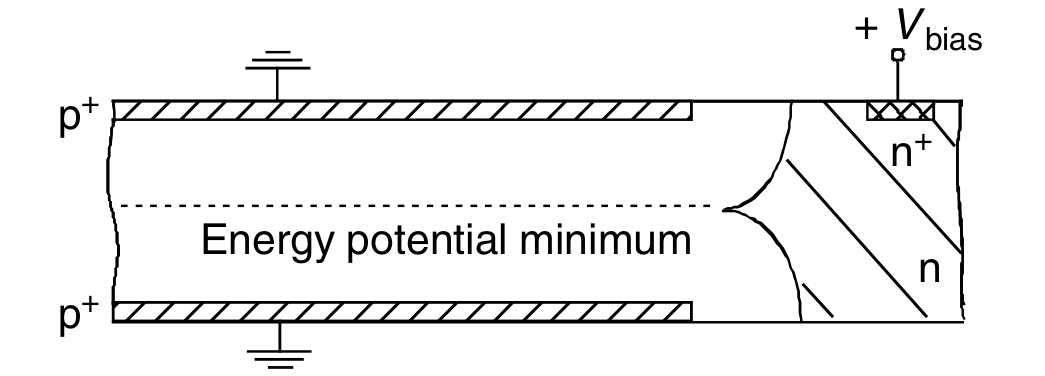
\includegraphics[width=0.85\textwidth]{illustrations/sdd_concept.png}
  \caption[Prinzip eines SDD]{Schematisch abgebildet ist das Wirkungsprinzip eines Silizum Drift Detektors. Von den gegenüberliegenden p-Elektroden bildet sich eine Vararmungszone seitwärts zur n-Elektrode hin aus \cite[S.~223, bearbeitet]{bbbook}.}
  \label{fig:sdd_concept}
\end{figure}

Außerdem wird durch konzentrische Ringe auf der Rückseite des SDD ein weiteres elektrisches Feld parallel zur Detektoroberfläche so angelegt, dass die durch die ionisierende Strahlung ausgelösten Elektronen seitlich zur n-Anode beschleunigt werden. Veranschaulicht kann man sich \cref{fig:sdd_concept} so vorstellen, dass die p-Elektroden senkrecht zur Oberfläche in kleinere Elemente zerlegt sind und zwischen diesen eine kleine Potentialdifferenz für die Beschleunigung, den Drift, der Elektronen sorgt. Später werden die Elektronenladungen durch einen Feldeffekttransistor in eine Spannung proportional zu den ausgelösten Elektronen und damit zur Photonenenergie der eintreffenden Röntgenstrahlung umgewandelt, welche nachfolgend von einem Multi-Channel-Analyser ausgewertet werden kann.



